


\documentclass{article}   


\usepackage{comment}
\usepackage{amsfonts}
\usepackage{amsmath}
\usepackage{amsthm}
% \usepackage{natbib}
\usepackage{graphicx} 
\usepackage{algpseudocode}
\usepackage{algorithmicx}
\usepackage{algorithm}
\usepackage{url}       
% \usepackage{subfig}
\usepackage{caption}
\usepackage{subcaption}
% \usepackage{fullpage}       

                             
  
                               \newcommand{\A}{\mathcal{A}}
                               \newcommand{\B}{\mathcal{B}}
                               \newcommand{\E}{\mathcal{E}}
                               \renewcommand{\H}{\mathcal{H}}
                               \renewcommand{\L}{\mathcal{L}}
                               \renewcommand{\P}{\mathcal{P}}
                               \newcommand{\Q}{\mathcal{Q}}
                               \newcommand{\U}{\mathcal{U}}
                               \newcommand{\V}{\mathcal{V}}
                               \newcommand{\C}{\mathbb{C}}
                               \newcommand{\I}{\mathbb{I}}
                               \newcommand{\N}{\mathbb{N}}
                               \newcommand{\R}{\mathbb{R}}
                               \newcommand{\T}{\mathbb{T}}
                               \newcommand{\Z}{\mathbb{Z}}
                               \newcommand{\argmin}{\operatorname*{argmin}}
                               \newcommand{\prox}{\operatorname{prox}}
                               
\newtheorem{thm}{Theorem}
\newtheorem{cor}{Corollary}
\newtheorem{lem}{Lemma}


	\addtolength{\oddsidemargin}{-1in}
	\addtolength{\evensidemargin}{-1in}
	\addtolength{\textwidth}{2in}

	\addtolength{\topmargin}{-1.25in}
	\addtolength{\textheight}{1.75in}

\begin{document}

\title{EE225E Project Proposal: \\
Metabolism mapping with prior information 
}
\author{John Maidens and Kamin Kahrizi}
% \date{April 13, 2016} 

\maketitle


\subsection{Dynamic metabolic MRI using hyperpolarized carbon-13 pyruvate}


Hyperpolarized carbon-13 magnetic resonance imaging (MRI) has enabled the real-time observation of perfusion and metabolism in preclinical and clinical studies. \cite{Golman06, Day07, Kazan13, Nelson13, Bahrami14, Swisher14}
This technology is made possible by techniques for dynamic nuclear polarization (DNP) that have led to signal-to-noise ratio (SNR) increases of four to five orders of magnitude compared with endogenous signal in dissolved $^{13}$C-labelled molecules  \cite{Ardenkjaer-Larsen03, Golman03}.  Injected [1-$^{13}$C] pyruvate is frequently used as a substrate in metabolism experiments and its rate of conversion to  [1-$^{13}$C] lactate has been shown to distinguish between healthy and diseased tissues in animal \cite{Day07}, and recently human \cite{Nelson13}, studies. 

In contrast with conventional MRI, hyperpolarized experiments are inherently dynamic as images must be acquired as the injected substrate spreads through the body and is metabolized. This necessitates dynamical system modelling and estimation for quantifying metabolic reaction rates. 

\subsection{Mathematical model} 

We consider a two-dimensional system of ordinary differential equations 
\begin{equation}
%  \resizebox{0.9\columnwidth}{!}{$
  \displaystyle \frac{dx}{dt}(t) =  \left[ \begin{array}{cc}
   -k_{PL} - R_{1P} & 0 \\ 
    k_{PL} & -R_{1L} \end{array} \right] x(t) +  \left[ \begin{array}{c} k_{TRANS} \\ 0 \end{array} \right] u(t)
%  $}
  \label{eq:ct}
\end{equation}
that models the magnetization dynamics in a tissue with an arterial input function $u(t)$ and uni-directional conversion from the substrate (pyruvate) to a metabolic product (lactate), which has been commonly applied for hyperpolarized $^{13}$C pyruvate experiments. The state $x_1(t)$ denotes the longitudinal magnetization of pyruvate contained in a particular voxel in the tissue and $x_2(t)$ the longitudinal magnetization of lactate in the same voxel. The rate of metabolism of pyruvate to lactate is denoted $k_{PL}$, the perfusion rate from the arterial input to the tissue is denoted $k_{TRANS}$, and $R_{1P}$ and $R_{1L}$ are lumped parameters that account for T$_1$ decay in the magnetization along with other effects, such as metabolism of pyruvate into products other than lactate as well as flow of magnetization out of the slice. The input to the system $u(t)$ is an unmeasured arterial input function (AIF) resulting from the injection of hyperpolarized [1-$^{13}$C] pyruvate and is assumed to be of gamma-variate shape
 \[
   u(t) = A_0 (t - t_0)^\gamma e^{-(t -t_0)/\beta}. 
 \]
 
We acquire data at $N$ time points separated by intervals of length T$_R$. 
Each time $t$ an acquisition is made, we must choose a flip angle $\alpha_{k, t}$ for each compound $k$ to be
measured. If the magnetization of the $k$-th compound before the acquisition is $x_k$, then this choice of flip
angle allows us to measure a signal of magnitude $\sin(\alpha_{k, t}) x_k$, after which $\cos(\alpha_{k, t}) x_k$ magnetization
remains for future acquisitions. This causes discrete jumps, or resets, in the system state, leading to a hybrid dynamical system \cite{Lygeros08,Goebel12}. Since we are only interested in the system's state at acquisition times, we can avoid technicalities associated with hybrid system modelling by discretizing the system in time and considering a discrete-time dynamical system that simultaneously captures the  evolution of (\ref{eq:ct}) between acquisitions and the discrete jumps induced by the acquisitions. 
%Each time we acquire data, we choose a flip angle $\alpha_t$, allowing us to measure a signal of magnitude $\sin(\alpha_t) x_t$ in the transverse plane. After the acquisition, $\cos(\alpha_t) x_t$ magnetization remains in the longitudinal direction. 
We define the transition matrices $A_d$ and $B_d$
\begin{equation*}
%  \resizebox{\columnwidth}{!}{$
\begin{split}
  A_d &= \exp\left( T_R  \left[ \begin{array}{cc}
    -k_{PL} - R_{1P} & 0           \\ 
     k_{PL}                & -R_{1L} \end{array} \right] \right) \\
  B_d &= \left[ \begin{array}{cc}
    -k_{PL} - R_{1P} & 0           \\ 
     k_{PL}                & -R_{1L} \end{array} \right]^{-1}(A_d- I)   \left[ \begin{array}{c} k_{TRANS} \\ 0 \end{array} \right]
  \end{split}
%$}
\end{equation*}
that correspond to the discretization of (\ref{eq:ct}) assuming a zero-order hold on the input between each acquisition \cite{Chen98}.  

We will construct metabolite maps using magnitude image data. This allows us to avoid modelling sources of phase in the image and keeps the model dimension small, requiring only a single state for each metabolite. Accordingly, we model the measurements as independent Rician-distributed random variables \cite{Gudbjartsson95}, which have probability density
\[
   p_{x, \sigma}(y) =  \frac{y}{\sigma^2} \exp\left( - \frac{y^2 + x^2}{2 \sigma^2} \right) I_0\left(\frac{y x}{\sigma^2} \right)
\]
where $I_\nu$ denotes the modified Bessel function of the first kind of order $\nu$.  All together, we have the discrete-time model for the observed data from a single voxel: 
\begin{equation}
  % \resizebox{0.9\columnwidth}{!}{$
\begin{split}
 %  u_t(\theta) &= A_0 (tT_R-t_0)^\gamma e^{-\frac{t T_R -t_0}{\beta}}  \\
  x_0 &= 0 \\
  x_{t+1} &= A_d(\theta) \left[\begin{array}{cc} \cos \alpha_{1,t} & 0 \\  0 & \cos \alpha_{2, t} \end{array}\right]  x_t + B_d(\theta) u_t(\theta)  \\
 \tilde{x}_{k, t} &= \sin(\alpha_{k, t}) x_{k, t} \ \ \ k=1, 2 \\
  Y_{k, t} &\sim Rice(\tilde x_{k, t}, \sigma_k ) \ \ \ k = 1, 2. 
\end{split}
%  $}
\label{eq:model}
\end{equation}


\subsection{Low SNR degrades parameter map quality} 

Even with dynamic nuclear polarization, carbon-13 MRI suffers from low SNR relative to conventional MRI. This makes it difficult to acquire high-resolution images, as large voxel sizes are required to achieve sufficient SNR. 

In Figure \ref{fig:effect_of_resolution} we show the effect of increased resolution on the quality of parameter maps computed by an independent maximum-likelihood fit to each voxel. We generate data from the model given in equation (2) of \cite{Maidens16}, assuming that SNR of the trajectories of the model is proportional to voxel volume. We see that when voxels are treated independently (\emph{i.e} no spatial structure is assumed in the parameter maps) increased resolution can be detrimental to parameter map quality. 

\begin{figure} 
    \centering
    \begin{subfigure}[b]{0.25\textwidth}
        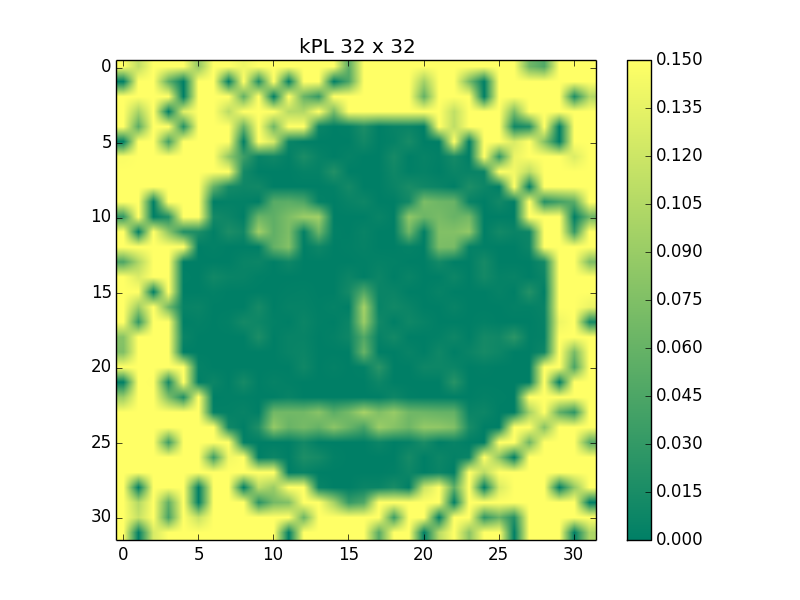
\includegraphics[width=\textwidth]{figs/kPL_32.png}
        \caption{$k_{PL}$: 32 $\times$ 32}
        % \label{fig:gull}
    \end{subfigure}
    ~ %add desired spacing between images, e. g. ~, \quad, \qquad, \hfill etc. 
      %(or a blank line to force the subfigure onto a new line)
    \begin{subfigure}[b]{0.25\textwidth}
        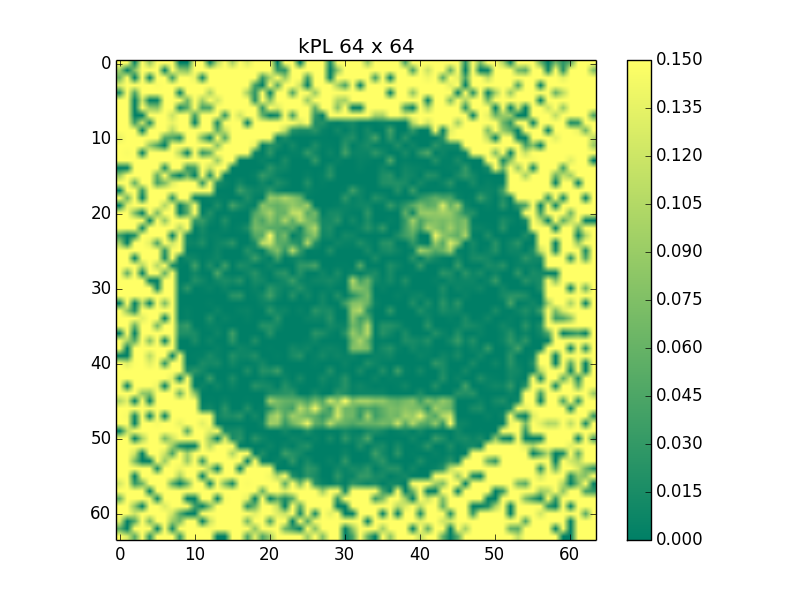
\includegraphics[width=\textwidth]{figs/kPL_64.png}
        \caption{$k_{PL}$: 64 $\times$ 64}
       %  \label{fig:tiger}
    \end{subfigure}
    ~ %add desired spacing between images, e. g. ~, \quad, \qquad, \hfill etc. 
    %(or a blank line to force the subfigure onto a new line)
    \begin{subfigure}[b]{0.25\textwidth}
        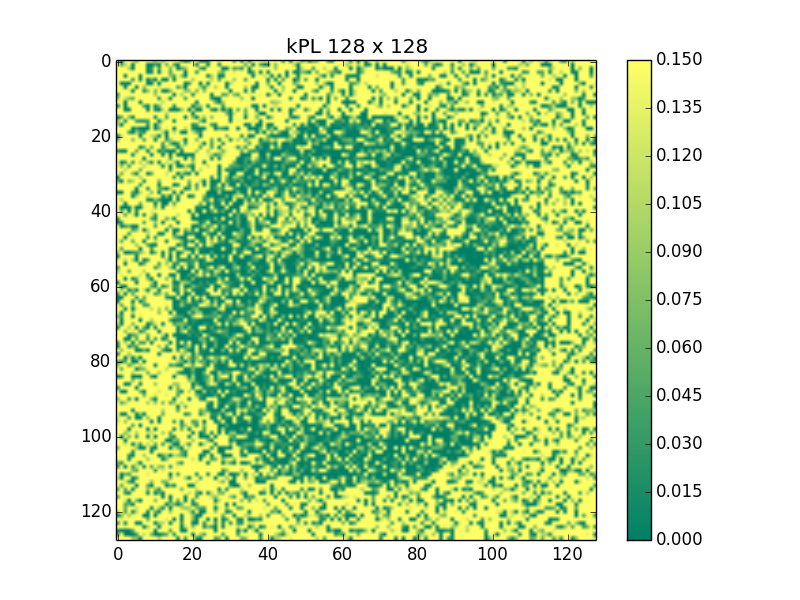
\includegraphics[width=\textwidth]{figs/kPL_128.png}
        \caption{$k_{PL}$: 128 $\times$ 128}
        % \label{fig:mouse}
    \end{subfigure}
    
        \begin{subfigure}[b]{0.25\textwidth}
        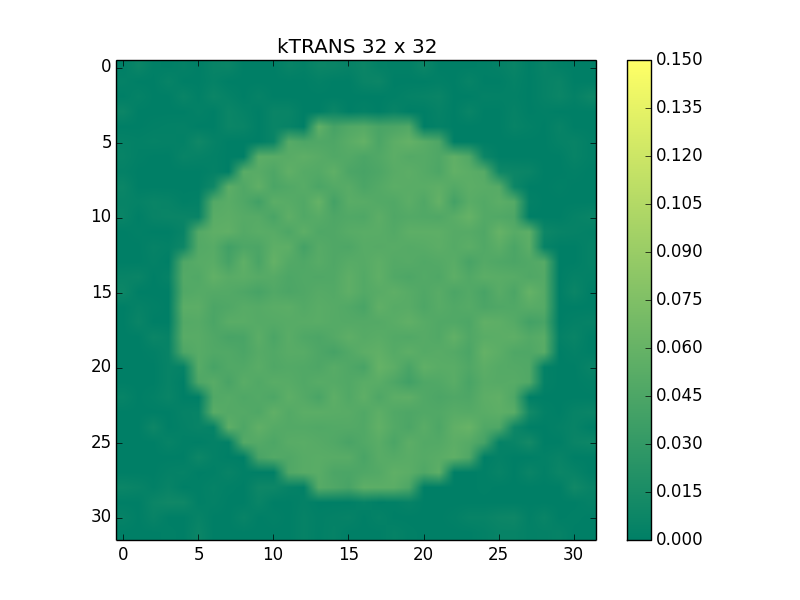
\includegraphics[width=\textwidth]{figs/kTRANS_32.png}
        \caption{$k_{TRANS}$: 32 $\times$ 32}
        % \label{fig:gull}
    \end{subfigure}
    ~ %add desired spacing between images, e. g. ~, \quad, \qquad, \hfill etc. 
      %(or a blank line to force the subfigure onto a new line)
    \begin{subfigure}[b]{0.25\textwidth}
        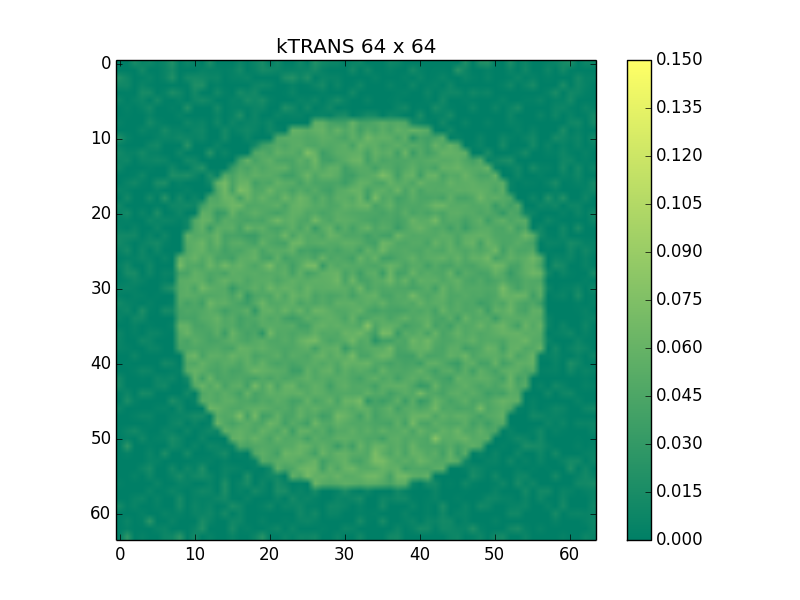
\includegraphics[width=\textwidth]{figs/kTRANS_64.png}
        \caption{$k_{TRANS}$: 64 $\times$ 64}
       %  \label{fig:tiger}
    \end{subfigure}
    ~ %add desired spacing between images, e. g. ~, \quad, \qquad, \hfill etc. 
    %(or a blank line to force the subfigure onto a new line)
    \begin{subfigure}[b]{0.25\textwidth}
        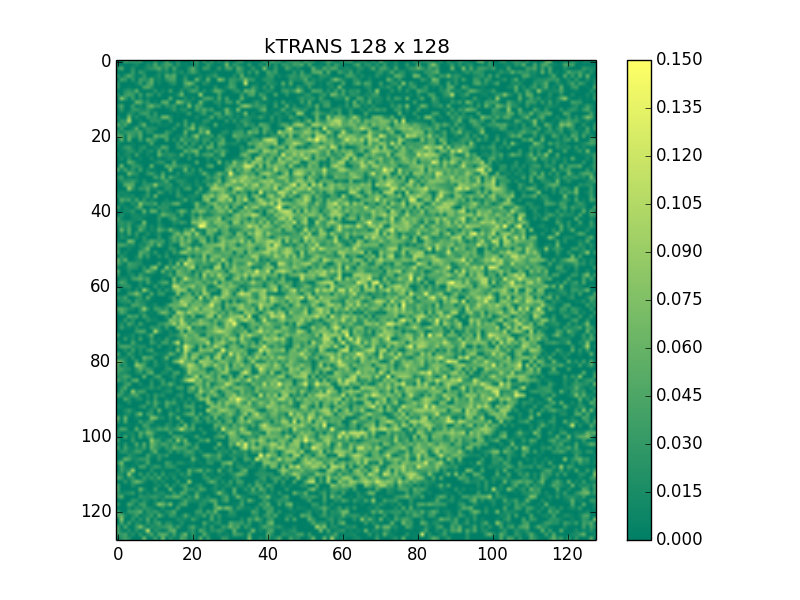
\includegraphics[width=\textwidth]{figs/kTRANS_128.png}
        \caption{$k_{TRANS}$: 128 $\times$ 128}
        % \label{fig:mouse}
    \end{subfigure}
    \caption{Parameter maps of varying resolution fit to simulated data sets. The first row shows parameter maps for the metabolic rate parameter $k_{PL}$; the second row shows parameter maps for the perfusion parameter $k_{TRANS}$. }\label{fig:effect_of_resolution}
\end{figure}

\subsection{Spatial regularization to improve parameter maps} 
In order to overcome this limitation, we propose to investigate incorporating prior information about parameter maps by including regularization in the mapping. This will allow spatial structure in the data to be exploited, which was ignored in the previous analysis. We hope that this will help to solve the problem of low SNR in high-resolution carbon-13 images. 

Let $y_i$ denote a dynamic dataset generated by the model given in equation (2) of \cite{Maidens16} corresponding to some voxel $i$ from the set of all voxels $\mathcal{V}$. We wish to solve the optimization problem  
\begin{equation}
\begin{split}
\textbf{minimize} & \quad  \sum_{i \in \mathcal{V}} -\ell(\theta_i | y_i) + \lambda r(\theta) 
\end{split} 
\label{eq:opt}
\end{equation} 
where $\ell(\theta_i | y_i)$ denotes the log likelihood function corresponding to the model and $r$ is a regularizer that corresponds to prior information we have about the parameter map. For example, for the parameter map in Figure \ref{fig:effect_of_resolution} we might use a total-variation regularization term in order to exploit the prior knowledge that the map is piecewise-constant. 


To solve \ref{eq:opt} we introduce $z = \theta$ and solve
\begin{equation}
\begin{split}
\textbf{minimize} & \quad  \sum_{i \in \mathcal{V}} -\ell(\theta_i | y_i) + \lambda r(z) \\
\textbf{subject to} & \quad \theta - z = 0
\end{split} 
\end{equation} 
This can be solved using the Douglas-Rachford iteration (a special case of ADMM) 
\[
\begin{split} 
\theta^{k+1} &= \argmin_\theta  \sum_{i \in \mathcal{V}} -\ell(\theta_i | y_i) + \frac{\rho}{2} \|\theta - z^k + u^k \|_2^2 \\
% &= \argmin_\theta  \sum_{i \in \mathcal{V}}\left[ -\ell(\theta_i | y_i) + \frac{\rho}{2} \|\theta_i - z_i^k + u_i^k \|_2^2 \right] \\
z^{k+1} &= \argmin_z \lambda r(z) + \frac{\rho}{2} \| \theta^{k+1} - z + u^k \|_2^2 \\
u^{k+1} &= u^k + \theta^{k+1} - z^{k+1}
\end{split} 
\]
Note that both the $\theta$ update is additively separable. Introducing the proximity operator
\[
\prox_f(x) = \argmin_u f(u) + \frac{1}{2} \|u - x\|_2^2 
\]
we can re-write this iteration as 
\[
\begin{split} 
\theta_i^{k+1} &= \prox_{-\frac{1}{\rho} \ell(\cdot | y_i)} (z_i^k - u_i^k) \quad i \in \mathcal{V} \\
z^{k+1} &= \prox_{\frac{\lambda}{\rho} r} (\theta^{k+1} + u^k) \\
u^{k+1} &= u^k + \theta^{k+1} - z^{k+1}. 
\end{split} 
\]

\subsection{Linear least-squares method for $k_{PL}$ mapping} 

An alternative approach is to try to fit parameter values to the model \eqref{eq:ct} directly. This model is linear in the parameter vector $\theta = [k_{TRANS} \quad k_{PL}]^T$, assuming that $x(t)$, $u(t)$ and $\frac{dx}{dt}(t)$ are all known. That is, we can rewrite \eqref{eq:ct} as 
\[
M(t) \theta = \left[\begin{array}{rr} u(t) & -P(t) \\ 0 & P(t) \end{array}\right] \left[\begin{array}{c} k_{TRANS} \\ k_{PL} \end{array}\right] = \left[\begin{array}{c} \dot P(t) + R_{1P}P(t) \\ \dot L(t) + R_{1L}L(t)\end{array}\right] = b(t).  
\]
Stacking estimates of $M(t)$ and $b(t)$ for various acquisition times $t_k$ into matrices $M$ and $b$ respectively, we can then estimate $\theta$ by solving the linear equation
\begin{equation}
M \theta = b
\end{equation} 
in the least squares sense. 

\subsection{Project goals:}
\begin{itemize}
\item Explore whether similar things have been done before (\emph{e.g.} in dynamic contrast enhanced MRI). 
\item Implement a Douglas-Rachford iteration to try to solve \eqref{eq:opt} and investigate convergence properties (since the negative log likelihood in this case in non-convex). 
\item Investigate applying to more realistic simulated data sets (\emph{e.g.} subsampled k-space). 
\item Write a 10 page report summarizing results. 
\end{itemize} 

\bibliographystyle{IEEEtran}
\bibliography{hyperpolarized}

\end{document}
